\lecture{24}{14 maggio 2024}
\section{Sistemi ottici}
Si parla di sistemi ottici quando più superfici ottiche (catottiche o diottriche) concorrono a formare una immagine di un oggetto.

\subsection{Lenti sottili vicine}
Considero due lenti sottili con lo stesso asse ottico collocate vicine, a distanza L piccola rispetto alle rispettive focali. Le equazioni delle due lenti sono
\begin{align}
	\frac{1}{p}+\frac{1}{q^{\prime} } &= \frac{1}{f_1}
	&
	\frac{1}{p^{\prime} } + \frac{1}{q} &= \frac{1}{f_2}
\end{align}
Si ha anche \(q^{\prime} +p^{\prime} =L\) che, per \(L\to 0\) dà \(p^{\prime} = -q^{\prime} \).
\begin{figure}[H]
	\centering
	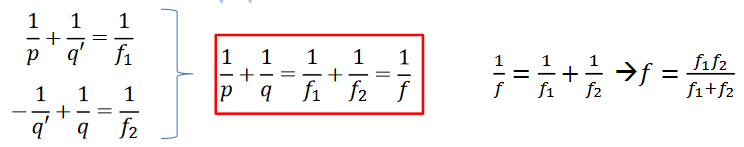
\includegraphics[width=0.6\textwidth]{screenshots/2024-05-14-11-21-41.png}
\end{figure}
Due lenti sottili vicine si comportano come una lente singola di opportuna focale. È importante perché dall'equazione dei costruttori di lenti sappiamo che \(f_{1,2}(n)\) e \(f_{1,2}(\lambda )\), quindi scegliendo materiali diversi ed opportuni si può minimizzare la dipendenza di \(f\) da \(\lambda \) per ottenere delle lenti acromatiche.

\subsection{Microscopio ottico}
Il microscopio ottico è costruito per produrre immagini alla distanza migliore per la visione, che è di circa \SI{25}{cm}. È composto da una lente obiettivo convergente a focale ridotta e una oculare a focale maggiore.
\begin{figure}[H]
	\centering
	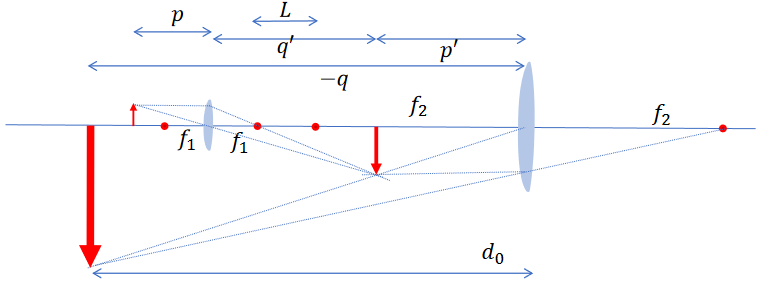
\includegraphics[width=0.6\textwidth]{screenshots/2024-05-14-11-27-47.png}
\end{figure}
Le equazioni delle lenti sono le stesse di prima:
\begin{align}
	\frac{1}{p} + \frac{1}{q^{\prime} } &= \frac{1}{f_1}
	&
	\frac{1}{p^{\prime} } + \frac{1}{q} &= \frac{1}{f_2}
\end{align}
Le coordinate sono legate da questa relazione: \(q^{\prime} + p^{\prime} = L + f_1 + f_2\). Scelgo \(L= \SI{16}{cm} \), \(q\equiv d_0 = \SI{25}{cm} \), \(f_1 \ll f_2 < L\). Inoltre con buona approssimazione ho \(p\thickapprox f_1,\ p^{\prime} \thickapprox f_2,\ q^{\prime} =L+f_1 +f_2 -p^{\prime} \thickapprox L + f_1 \thickapprox L\). L'ingrandimento complessivo risulta \(G=m_1 m_2 \thickapprox \frac{q^{\prime} }{p} \frac{q}{p^{\prime} } = \frac{d_0 L}{f_1 f_2}\). Gli ingrandimenti ragionevoli per i microscopi ottici vanno da 10x a 1000x. Ci sono diversi limiti fisici a questa tecnologia: il primo è la diffrazione. La nostra pupilla può vedere come distinti punti distanti \SI{0.1}{mm} a \SI{25}{cm} di distanza. Inoltre una struttura di \SI{1}{\micro \metre} appare grande \SI{1}{mm}, quindi non posso vedere la sua struttura interna. Serve il microscopio elettronico.

\subsection{Telescopio rifrattore}
La luce che arriva da molto lontano viaggia per raggi paralleli. Il sistema ottico del telescopio è costituito da una lente obiettivo convergente a focale lunga e una oculare convergente a focale più piccola. Il fuoco della prima lente coincide con il fuoco della seconda.
\begin{figure}[H]
	\centering
	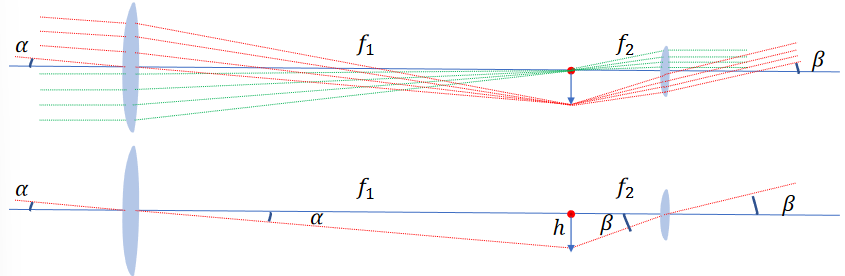
\includegraphics[width=0.6\textwidth]{screenshots/2024-05-14-11-40-57.png}
\end{figure}
Si definisce l'ingrandimento angolare
\begin{equation}
	M = \frac{\beta }{\alpha } = \frac{\tan \beta }{\tan \alpha } = \frac{h}{f_2} \frac{f_1}{h} = \frac{f_1}{f_2}
\end{equation}
Il sistema inverte l'alto con il basso e la destra con la sinistra. Posso sostituire la seconda lente con una lente oculare divergente a focale piccola. Il fuoco della prima lente coincide con il secondo fuoco della seconda. (È il cannocchiale galileiano).
\begin{figure}[H]
	\centering
	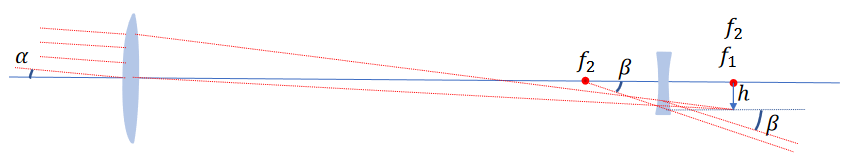
\includegraphics[width=0.6\textwidth]{screenshots/2024-05-14-11-46-31.png}
\end{figure}
Così il sistema non è invertente. L'ingrandimento angolare è \(M=\frac{\beta }{\alpha } = \frac{\tan \beta }{\tan \alpha } = \frac{h}{\vert f_2 \vert } \frac{f_1}{h} = \frac{f_1}{\vert f_2 \vert }\).

L'alternativa è usare una "lente di Barlow". Per costruire il cannocchiale terrestre si può aggiungere al telescopio rifrattore una lente di Barlow (fra la prima e la seconda lente) per ribaltare l'immagine. La lente di Barlow è una singola lente convergente a focale piccola (\num{2}-\SI{4}{cm}) e un oggetto a \(p=2f\). L'ingrandimento angolare è 1.
\begin{figure}[H]
	\centering
	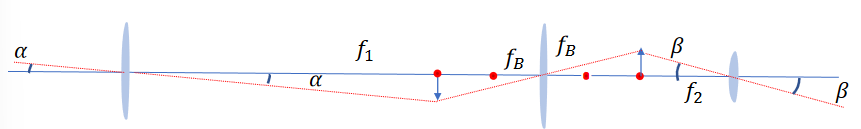
\includegraphics[width=0.7\textwidth]{screenshots/2024-05-14-11-49-54.png}
\end{figure}

I binocoli comuni sono costituiti dal telescopio rifrattore e da un sistema per ribaltare le immagini costituito da prismi.

\subsection{Aberrazioni}
Si indica con "aberrazione" la differenza tra ciò che si voleva ottenere con un sistema ottico e l'immagine effettivamente ottenuta. Le differenze nascono dalle varie approssimazioni che sono state fatte nella derivazione delle formule dell'ottica. Si può avere aberrazione cromatica dovuta alla dipendenza di \(f\) dall'indice di rifrazione e dalla lunghezza d'onda. Si può avere aberrazione sferica con i raggi che passano vicini ai bordi della lente. Si risolve usando lenti a grandi raggi e ponendoci davanti un diaframma. Posso avere anche aberrazione di coma quando raggi non parassiali vengono focalizzati in punti diversi. Si può avere anche distorsione a cuscino (ingrandimento maggiore in periferia dell'immagine) o distorsione a barile (ingrandimento maggiore al centro). Nelle slide si trovano immagini di esempio di questi fenomeni.